\documentclass[11pt,a4paper]{article}

\usepackage[a4paper,top=17mm,bottom=18mm,left=19mm,right=19mm,headheight=14pt]{geometry}
\usepackage{fontspec}
\usepackage{graphicx}
\usepackage{booktabs}
\usepackage{tabularx}
\usepackage{array}
\usepackage{amsmath}
\usepackage{microtype}
\usepackage{setspace}
\usepackage{enumitem}
\usepackage{xcolor}
\usepackage{caption}
\usepackage{fancyhdr}
\usepackage{titlesec}
\usepackage{tikz}
\usepackage[hidelinks]{hyperref}

\defaultfontfeatures{Ligatures=TeX}
\setmainfont{Times New Roman}
\setsansfont{Arial}
\newfontfamily\banglafont[Script=Bengali]{Nirmala UI}
\newcommand{\bn}[1]{{\banglafont #1}}

\definecolor{kuetgreen}{HTML}{007A42}
\definecolor{navy}{HTML}{173F67}
\definecolor{softgray}{HTML}{F2F4F6}
\definecolor{rulegray}{HTML}{6B7280}

\setstretch{1.06}
\setlength{\parindent}{0pt}
\setlength{\parskip}{4pt}
\setlist[itemize]{leftmargin=5mm,itemsep=1.5pt,topsep=2pt}
\captionsetup{font=small,labelfont=bf,skip=4pt}
\titleformat{\section}{\large\bfseries\color{navy}}{\thesection}{0.55em}{}[\vspace{-2pt}\color{rulegray}\titlerule]
\titleformat{\subsection}{\normalsize\bfseries\color{kuetgreen}}{\thesubsection}{0.45em}{}
\titlespacing*{\section}{0pt}{7pt}{4pt}
\titlespacing*{\subsection}{0pt}{5pt}{2pt}

\pagestyle{fancy}
\fancyhf{}
\fancyhead[L]{\footnotesize CSE 4122: Natural Language Processing Laboratory}
\fancyhead[R]{\footnotesize Bangla Punctuation Restoration}
\fancyfoot[C]{\thepage}
\renewcommand{\headrulewidth}{0.35pt}
\renewcommand{\footrulewidth}{0pt}

\newcommand{\metric}[1]{\textbf{#1}}
\newcolumntype{Y}{>{\centering\arraybackslash}X}
\newcolumntype{L}{>{\raggedright\arraybackslash}X}

\begin{document}

% -----------------------------------------------------------------------------
% Cover page
% -----------------------------------------------------------------------------
\begin{titlepage}
\thispagestyle{empty}
\begin{tikzpicture}[remember picture,overlay]
  \draw[line width=0.7pt] ([xshift=7mm,yshift=-7mm]current page.north west)
  rectangle ([xshift=-7mm,yshift=7mm]current page.south east);
\end{tikzpicture}

\begin{center}
\vspace*{11mm}
{\LARGE\bfseries Khulna University of Engineering \& Technology\par}
\vspace{2mm}
{\Large\bfseries Department of Computer Science and Engineering\par}

\vspace{5mm}

\includegraphics[height=28mm]{assets/kuet_logo.png}

\vspace{5mm}
{\Large\bfseries CSE 4122: Natural Language Processing Laboratory\par}

\vspace{10mm}
{\Large\bfseries Project Report on\par}
\vspace{4mm}
{\LARGE\bfseries Bangla Punctuation Restoration Using BERT and BiLSTM\par}
\vspace{1.5mm}
% {\LARGE\bfseries Platform for E-Commerce Sellers\par}

\vspace{13mm}
{\Large\bfseries Submitted by:\par}
\vspace{3mm}
{\large\bfseries MD Rahul Sheikh, 2107063\par}
\vspace{1.5mm}
{\large\bfseries Rezuan Mustafa Hasan, 2107075\par}
\vspace{3mm}
{\large\bfseries Year: 4th \qquad Term: 1st\par}

\vspace{10mm}
{\Large\bfseries Submitted to:\par}
\vspace{3mm}
{\large\bfseries Dr. K. M. Azharul Hasan\par}
{\normalsize Professor, Department of Computer Science and Engineering\par}
\vspace{4mm}
{\large\bfseries Md Nazirul Hasan Shawon\par}
{\normalsize Assistant Professor, Department of Computer Science and Engineering\par}

\vfill
{\large\textbf{Date of Submission:} September 23, 2026\par}
\vspace{8mm}
\end{center}
\end{titlepage}

\setcounter{page}{1}

% -----------------------------------------------------------------------------
% Page 1: motivation and task definition
% -----------------------------------------------------------------------------
\section{Abstract}
Bangla text written in reviews, messages, and informal documents often omits punctuation. This report presents the project's core NLP component: restoring punctuation in an unpunctuated Bangla word sequence. Two models implement the same gap-classification task. The first fine-tunes an aligned BanglaBERT encoder and obtains strong contextual representations. The second combines frozen 300-dimensional fastText vectors with a packed, two-layer bidirectional LSTM (BiLSTM), producing a much smaller model. Both predict up to four ordered marks at every word boundary from eight punctuation symbols plus a STOP class. On the recorded validation set of 37,044 sentences, BanglaBERT achieved 68.58\% macro-F1 and 83.74\% exact match, while the BiLSTM achieved 50.32\% and 77.81\%. The results show a clear accuracy-efficiency trade-off: contextual pretraining improves difficult and rare marks, whereas the BiLSTM remains useful when storage and computation are limited.

\section{Introduction}
Punctuation communicates sentence boundaries, questions, emphasis, lists, and parenthetical structure. When it is removed, the words are still present but the reader must infer these relationships. Automatic restoration is therefore a sequence prediction problem: the system must examine the words on both sides of a boundary and decide whether one or more punctuation marks belong there.

The project compares two complementary approaches. BanglaBERT uses knowledge learned from a large Bangla corpus and builds a context-dependent vector for each word. The fastText-BiLSTM model starts with fixed word vectors and learns sequential patterns through forward and backward recurrent passes. To keep the comparison fair, both models use the same boundary representation, label vocabulary, four-slot output head, loss family, and evaluation contract.

\section{Problem Formulation}
For a sentence containing $N$ words, $w_1,\ldots,w_N$, the system defines $N+1$ gaps: one before the first word, one after the last word, and one between every adjacent pair. Each gap has four ordered slots. A slot predicts one of nine classes:
\[
\mathcal{C}=\{\text{STOP},\ \text{\bn{।}},\ \texttt{,},\ \texttt{?},\ \texttt{!},\ \texttt{;},\ \texttt{:},\ \texttt{(},\ \texttt{)}\}.
\]
STOP means that no further mark should be emitted for that gap. Thus a comma-only gap is encoded as $[\text{comma},\text{STOP},\ldots]$, while an empty gap begins with STOP. Labels after STOP are ignored during training. This representation supports short punctuation sequences without requiring an autoregressive decoder.

\begin{figure}[h]
\centering
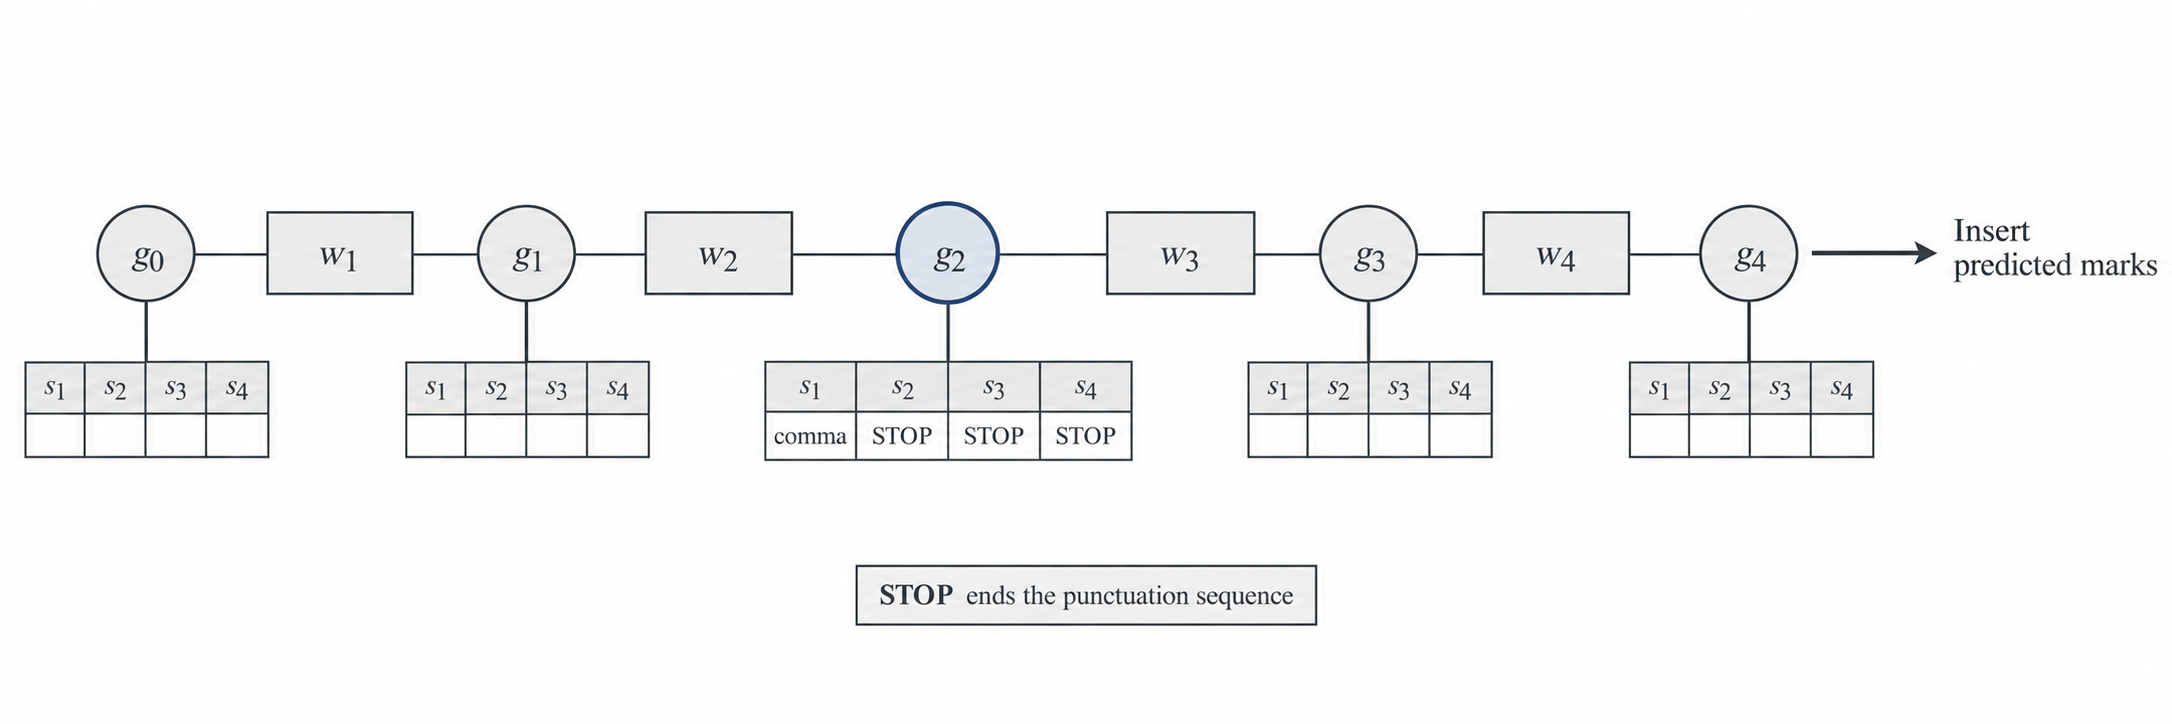
\includegraphics[width=0.98\linewidth]{assets/gap_annotation.png}
\caption{Gap-based prediction with four ordered slots. For four words, five boundary gaps are classified.}
\end{figure}

\clearpage

% -----------------------------------------------------------------------------
% Page 2: shared pipeline and BanglaBERT
% -----------------------------------------------------------------------------
\section{Shared Processing Pipeline}
Training text is first parsed into words and punctuation gaps. The punctuation is removed from the encoder input and retained only as target labels. Each model then produces a vector for every word, inserts learned beginning-of-sequence (BOS) and end-of-sequence (EOS) representations, and constructs one vector per gap from its left and right neighbors. A shared-style head maps each gap vector to $4\times9=36$ logits. At inference time, the highest-scoring class is selected in each slot and decoding stops at the first STOP. The predicted marks are finally inserted back into their original gaps.

\begin{figure}[h]
\centering
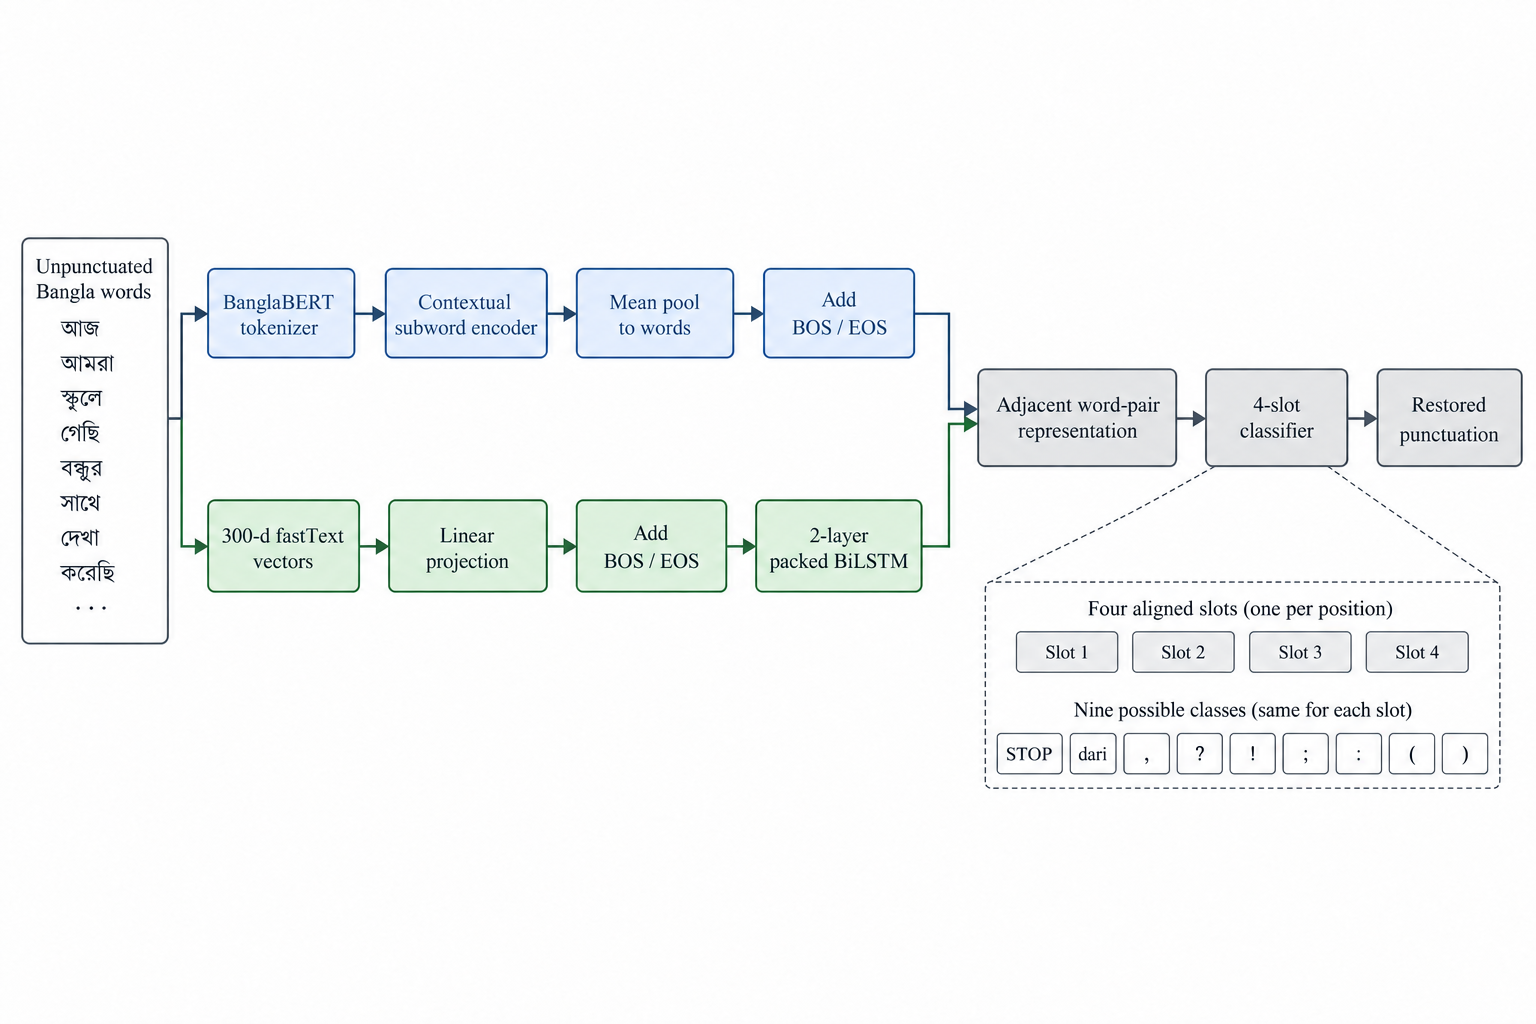
\includegraphics[width=0.99\linewidth,trim=0 195 0 195,clip]{assets/model_architecture.png}
\caption{The two encoder paths and their common adjacent-word, four-slot classification design.}
\end{figure}

\section{Model 1: Aligned BanglaBERT}
\subsection{Contextual encoding}
The model uses \texttt{csebuetnlp/banglabert}, an ELECTRA-style Bangla encoder. ELECTRA pretraining teaches a discriminator to detect replaced tokens, so a learning signal is available at every token position rather than only at masked positions \cite{electra}. BanglaBERT was pretrained using the Bangla2B+ corpus and reported strong results on the BLUB benchmark \cite{banglabert}. Fine-tuning adapts these general contextual features to punctuation restoration.

The tokenizer may split one word into several subwords. Labels, however, are defined for word gaps. The implementation therefore records each subword's original word index and mean-pools the corresponding 768-dimensional hidden vectors:
\[
h_i=\frac{1}{|S_i|}\sum_{j\in S_i} z_j,
\]
where $S_i$ is the set of subwords belonging to word $i$ and $z_j$ is a contextual subword vector. This explicit alignment prevents a single Bangla word from accidentally receiving several gap predictions.

\subsection{Boundary classification}
Learned BOS and EOS vectors are placed immediately around the real words, not around padding. For gap $i$, the model concatenates the contextual vectors on its two sides and projects the result:
\[
r_i=\operatorname{LayerNorm}\!\left(\operatorname{Dropout}\left(\operatorname{GELU}\left(W_g[h_i;h_{i+1}]+b_g\right)\right)\right).
\]
Here the concatenated vector has 1,536 values and the projection has 384. A final linear layer produces 36 logits, reshaped to four slots by nine classes. Because BanglaBERT sees the whole sequence through self-attention, the representation of a boundary can include both nearby syntax and more distant sentence context.

\clearpage

% -----------------------------------------------------------------------------
% Page 3: BiLSTM and training
% -----------------------------------------------------------------------------
\section{Model 2: Packed fastText-BiLSTM}
\subsection{Word representation and recurrence}
This model uses a frozen 300-dimensional fastText vector for each word. fastText represents words with character subword information, which is helpful for morphologically varied or uncommon spellings \cite{fasttext}. A learned linear layer projects each vector from 300 to 384 dimensions, followed by dropout. Learned BOS and EOS vectors then frame the real sentence.

The sequence enters a two-layer bidirectional LSTM \cite{lstm}. Each direction has 192 hidden units, so the forward and backward states together form a 384-dimensional vector at every position. The forward LSTM summarizes evidence from the left, while the backward LSTM summarizes evidence from the right. This is a natural fit for punctuation: a comma or question mark often depends on words appearing on both sides of a boundary.

Sentences in a batch have different lengths. Ordinary padded recurrence may let artificial zero tokens influence hidden states. The implementation instead applies \texttt{pack\_padded\_sequence} to lengths $N+2$, including BOS and EOS. The LSTM processes only real positions; the output is unpacked afterward. EOS is placed immediately after each sentence's final word, never after batch padding.

As in BanglaBERT, adjacent 384-dimensional outputs are concatenated into 768 values, projected back to 384 with GELU, dropout, and layer normalization, and classified into 36 logits. The identical output design makes model comparison meaningful.

\section{Training Procedure}
The target distribution is strongly imbalanced: the dari and comma occur much more often than exclamation marks, semicolons, colons, or parentheses. Both recorded runs use smoothed inverse-frequency class weights with power $0.5$ and a maximum weight of $6.0$. STOP retains normal weight. The optimized objective is weighted cross-entropy over all valid gap slots:
\[
\mathcal{L}=-\frac{1}{M}\sum_{m=1}^{M}\alpha_{y_m}\log p(y_m\mid x),
\]
where ignored trailing slots and padded gaps are excluded, $M$ is the number of valid slots, and $\alpha_{y_m}$ is the class weight.

Optimization uses AdamW, a 10\% linear warmup followed by cosine decay, weight decay of 0.01 where applicable, and gradient-norm clipping at 1.0. The checkpoint with the highest validation macro-F1 is retained. Seed 42 is recorded for both models.

\begin{table}[h]
\centering
\caption{Recorded training configuration and model scale.}
\small
\begin{tabularx}{\linewidth}{@{}Lcc@{}}
\toprule
\textbf{Setting} & \textbf{Aligned BanglaBERT} & \textbf{Packed fastText-BiLSTM} \\
\midrule
Epochs / batch size & 3 / 32 & 4 / 64 \\
Learning rate & $1\times10^{-5}$ & $1\times10^{-4}$ \\
Dropout / warmup ratio & 0.1 / 0.1 & 0.1 / 0.1 \\
Encoder width & 768 & 384 (192 per direction) \\
Gap projection & 1,536 $\rightarrow$ 384 & 768 $\rightarrow$ 384 \\
Approx. trainable parameters & 110.4 million & 2.2 million \\
Checkpoint size in this project & 422.1 MiB & 8.4 MiB \\
\bottomrule
\end{tabularx}
\end{table}

\clearpage

% -----------------------------------------------------------------------------
% Page 4: results
% -----------------------------------------------------------------------------
\section{Evaluation and Results}
The reported measures answer different questions. \textit{Macro-F1} averages F1 equally across the eight punctuation symbols, so rare marks matter. \textit{Micro-F1} combines all decisions and is influenced by frequent marks. \textit{Ordered exact match} requires a complete sentence's predicted gap sequences to match the gold annotation. Parenthesis span F1 evaluates correctly paired opening and closing boundaries. The false-parenthesis rate counts negative sentences that incorrectly receive parentheses, normalized per 1,000 negatives.

The validation set contains 37,044 sentences. The retained benchmark contains 185,370 sentences, but the supplied benchmark report identifies it as reused exploratory evaluation rather than an untouched final test set. Consequently, these values support comparison between the frozen candidates under the same scoring contract, but they should not be presented as a new unbiased generalization estimate.

\begin{table}[h]
\centering
\caption{Validation F1 by punctuation symbol.}
\small
\begin{tabular}{@{}lrrrrrrrr@{}}
\toprule
\textbf{Model} & \bn{।} & \textbf{,} & \textbf{?} & \textbf{!} & \textbf{;} & \textbf{:} & \textbf{(} & \textbf{)} \\
\midrule
BanglaBERT & \textbf{98.95} & \textbf{84.47} & \textbf{94.25} & \textbf{26.15} & \textbf{26.85} & \textbf{67.32} & \textbf{75.80} & \textbf{74.85} \\
BiLSTM & 98.62 & 77.33 & 87.97 & 9.70 & 5.80 & 38.81 & 40.85 & 43.44 \\
\bottomrule
\end{tabular}
\end{table}

The two models are almost tied on the frequent dari, which is commonly a sentence-ending cue. The largest differences appear on marks requiring richer structural or semantic context. BanglaBERT improves colon F1 by 28.51 points and opening-parenthesis F1 by 34.95 points on validation. It also produces far fewer false parenthesis predictions. Rare exclamation marks and semicolons remain difficult for both models because their supports are only 433 and 87, respectively, compared with 35,723 dari instances and 19,223 commas.

The improvement is not only an effect of frequent symbols: BanglaBERT's macro-F1 advantage on the retained benchmark is 16.88 points. However, it requires about 50 times more trainable parameters and a checkpoint roughly 50 times larger. The BiLSTM therefore sacrifices accuracy for a substantially smaller footprint.

\clearpage

% -----------------------------------------------------------------------------
% Page 5: interpretation, limitations, conclusion, references
% -----------------------------------------------------------------------------
\section{Discussion}
BanglaBERT performs best because each word vector changes with the complete sentence. The same word can signal different punctuation in a question, a list, or a parenthetical phrase, and self-attention can connect distant evidence. Subword-to-word mean pooling is essential: it preserves pretrained subword knowledge while returning to the word-level gaps used by the task.

The BiLSTM remains a strong lightweight alternative. Its recurrent inductive bias follows word order directly, and bidirectionality provides left and right context without a large pretrained transformer. Packing is more than a speed optimization: it protects the sentence-final representation from padding contamination. Its frozen fastText input also reduces the number of trainable parameters. The cost is that a static word vector cannot adapt its meaning to the sentence as richly as BanglaBERT.

For an accuracy-first setting, aligned BanglaBERT is the appropriate default. For storage-limited, CPU-oriented, or offline use, the 8.4 MiB BiLSTM may be preferable if lower rare-mark and parenthesis accuracy is acceptable.

\section{Limitations and Future Work}
\begin{itemize}
  \item The retained benchmark was reused during the broader experimental process. A separately collected, untouched test set is needed for a final generalization claim.
  \item Rare classes dominate the remaining macro-F1 error. More balanced Bangla data, targeted augmentation, or focal loss could improve exclamation marks, semicolons, and colons.
  \item Four slots impose a fixed maximum punctuation sequence length. This is practical for the current corpus but should be checked when transferring to new domains.
  \item Parentheses are predicted locally even though they form paired structures. A constrained decoder or auxiliary span objective could enforce balanced pairs more directly.
  \item Future experiments should report repeated seeds, CPU/GPU latency, memory use, calibration, and qualitative error categories in addition to aggregate F1.
\end{itemize}

\section{Conclusion}
The project formulates Bangla punctuation restoration as word-gap classification with four ordered output slots. The two models share this formulation but differ in how they encode words. Aligned BanglaBERT uses pretrained contextual information and explicit subword-to-word pooling, yielding the strongest performance, especially for rare and structural punctuation. The packed fastText-BiLSTM uses static embeddings and bidirectional recurrence, giving a much smaller model with competitive results on frequent marks. Together, the models demonstrate a clear and practical trade-off between linguistic accuracy and computational cost.

\small
\begin{thebibliography}{9}
\setlength{\itemsep}{3pt}
\bibitem{banglabert} A. Bhattacharjee et al., ``BanglaBERT: Language Model Pretraining and Benchmarks for Low-Resource Language Understanding Evaluation in Bangla,'' \textit{Findings of NAACL}, pp. 1318--1327, 2022. DOI: \href{https://doi.org/10.18653/v1/2022.findings-naacl.98}{10.18653/v1/2022.findings-naacl.98}.

\bibitem{electra} K. Clark, M.-T. Luong, Q. V. Le, and C. D. Manning, ``ELECTRA: Pre-training Text Encoders as Discriminators Rather Than Generators,'' \textit{ICLR}, 2020.

\bibitem{fasttext} P. Bojanowski, E. Grave, A. Joulin, and T. Mikolov, ``Enriching Word Vectors with Subword Information,'' \textit{Transactions of the ACL}, vol. 5, pp. 135--146, 2017.

\bibitem{lstm} S. Hochreiter and J. Schmidhuber, ``Long Short-Term Memory,'' \textit{Neural Computation}, vol. 9, no. 8, pp. 1735--1780, 1997.

\bibitem{dossier} Project model dossier, source code, run configurations, validation metrics, and retained-benchmark report supplied in \texttt{report\_materials/}, accessed September 2026.
\end{thebibliography}

\end{document}
